
%%%%%%%%%%%%%%%%%%%%%%%%%%%%%%%%%%%%%%%%%%%%%%%%%%%%%%%%%%%%%%%%%%%%%%%%%%%%%%%%
%% CAPITULO
%%%%%%%%%%%%%%%%%%%%%%%%%%%%%%%%%%%%%%%%%%%%%%%%%%%%%%%%%%%%%%%%%%%%%%%%%%%%%%%%
\chapterimage{chapter_head_2.pdf} % Chapter heading image

\chapter{\textcolor{blue}{Historia do samba de gafieira}}
\label{cap:sambagafieira}
\index{Historia do samba de gafieira}


\section{Lundu} 
\label{sec:lundu}
\index{Dança!Lundu}
Esta é uma dança, brasileira, de roda e umbigada; esta teve sua origem no batuque dos bantos africanos,
e provavelmente trazida de Angola pelos escravos na segunda metade do século XVIII \cite[pp. 198]{dourado2004dicionario}.
Posteriormente foi introduzida aos salões das cortes do Brasil e Portugal.
No Brasil esta dança teve influencias da ``Modinha''(Portuguesa) e do ``Fandango''(Espanhol) \cite[pp. 198]{dourado2004dicionario}.



\section{Maxixe}
\label{sec:maxixe}
\index{Dança!Maxixe}
Esta é uma dança urbana afro-brasileira \cite[pp. 4]{musicasambavariasdef1}, 
em compasso binário, surgida em Rio de Janeiro, 
na Cidade Nova e nos cabarés de Lapa \cite[pp. 465]{marcondes1977enciclopedia}  \cite[pp. 198]{dourado2004dicionario}, 
aproximadamente entre 1870 e 1880 \cite[pp. 465]{marcondes1977enciclopedia}  \cite[pp. 62]{reinato2010musica}.

A dança era considerada de baixe ralé pela sociedade local, 
pois era entendida como um modismo indecente das classes baixas, imoral como o Lundu \cite[pp. 198]{dourado2004dicionario}.
Esta dança recebeu influencias da polca \cite[pp. 198]{dourado2004dicionario} e da Habanera \cite[pp. 62]{reinato2010musica}.

O maxixe tinha uma boa quantidade de passos como: 
parafuso, 
janela,
jocotó
saca-rolha, 
balão, 
balão apagado,
balão caindo,
corta-jaca,
urubu malandro,
sino, 
carrapeta, 
corta-capim, 
\cite[pp. 465]{marcondes1977enciclopedia} \cite[pp. 68, 129, 131,173]{efege1974maxixe} etc. 
Num principio o maxixe era dançado nas músicas de tango, havanera, polca e lundu; 
e só foi ate o final do século XIX que ganhou uma música com gênero próprio \cite[pp. 465]{marcondes1977enciclopedia}.

No inícios do século XX o maxixe foi exportado e dançado na Europa, atingindo um grande sucesso, 
chegando a ser apresentado pelo dançarino ``Duque'' em Paris (1914) e em Londres (1922) \cite[pp. 465]{marcondes1977enciclopedia}.
Este dançarino é considerado o civilizador do maxixe \cite[pp. 129]{efege1974maxixe}.

Uma explicação muito interessante do maxixe é cantada pela atriz, Aurélia Delorme,
numa representação num quadro de revista, interpretando  ``Maxixe Aristocrático'' (1904, José Nunes), 
que arrancava aplausos e provocava pedidos de bis;
o seguinte texto indica sua pauta \cite[pp. 80-81]{efege1974maxixe} \cite{REIS2003}: 
\begin{citando}
O maxixe tem ciência,\\
ou pelo menos tem arte.\\
Para haver proficiência\\
basta mexer certa parte.\\
Pois o próprio Padre Santo,\\
sabendo o gosto que tem,\\
virá de Roma ao Brasil\\
dançar maxixe também.\\ 
\end{citando}



\section{samba de gafieira}
O samba de gafieira, como dança, descende principalmente do maxixe (dança),
que a sua vez foi gerado  pela união do  lundu, 
a polca e outras danças europeias.
Assim, misturando o maxixe com a ginga, e o ritmo de outras danças africanas, 
é que se obteve o que agora chamaríamos como samba de gafieira (primigênio)\footnote{
Primitivo; primordial; o primeiro da sua espécie. = PRIMÍGENO \cite{priberamprimigenio}.
} \cite[pp. 139]{perna2002samba}.




A Figura \ref{fig:formuladosambagafieira} mostra a árvore genealógico do samba de gafieira (primigênio),
visto quando o samba fez sua aparição nos salões de dança denominados gafieiras.
\begin{figure}[h]
  \centering
  \begin{subfigure}[b]{0.535\textwidth}
    \centering
    \includegraphics[width=\textwidth]{chapters/cap-historia-sambagafieira/sambagafieiraformula.eps}
    \caption{Formação do samba de gafieira (primigênio).}
    \label{fig:formuladosambagafieira}
  \end{subfigure}
  \begin{subfigure}[b]{0.385\textwidth}
    \centering
    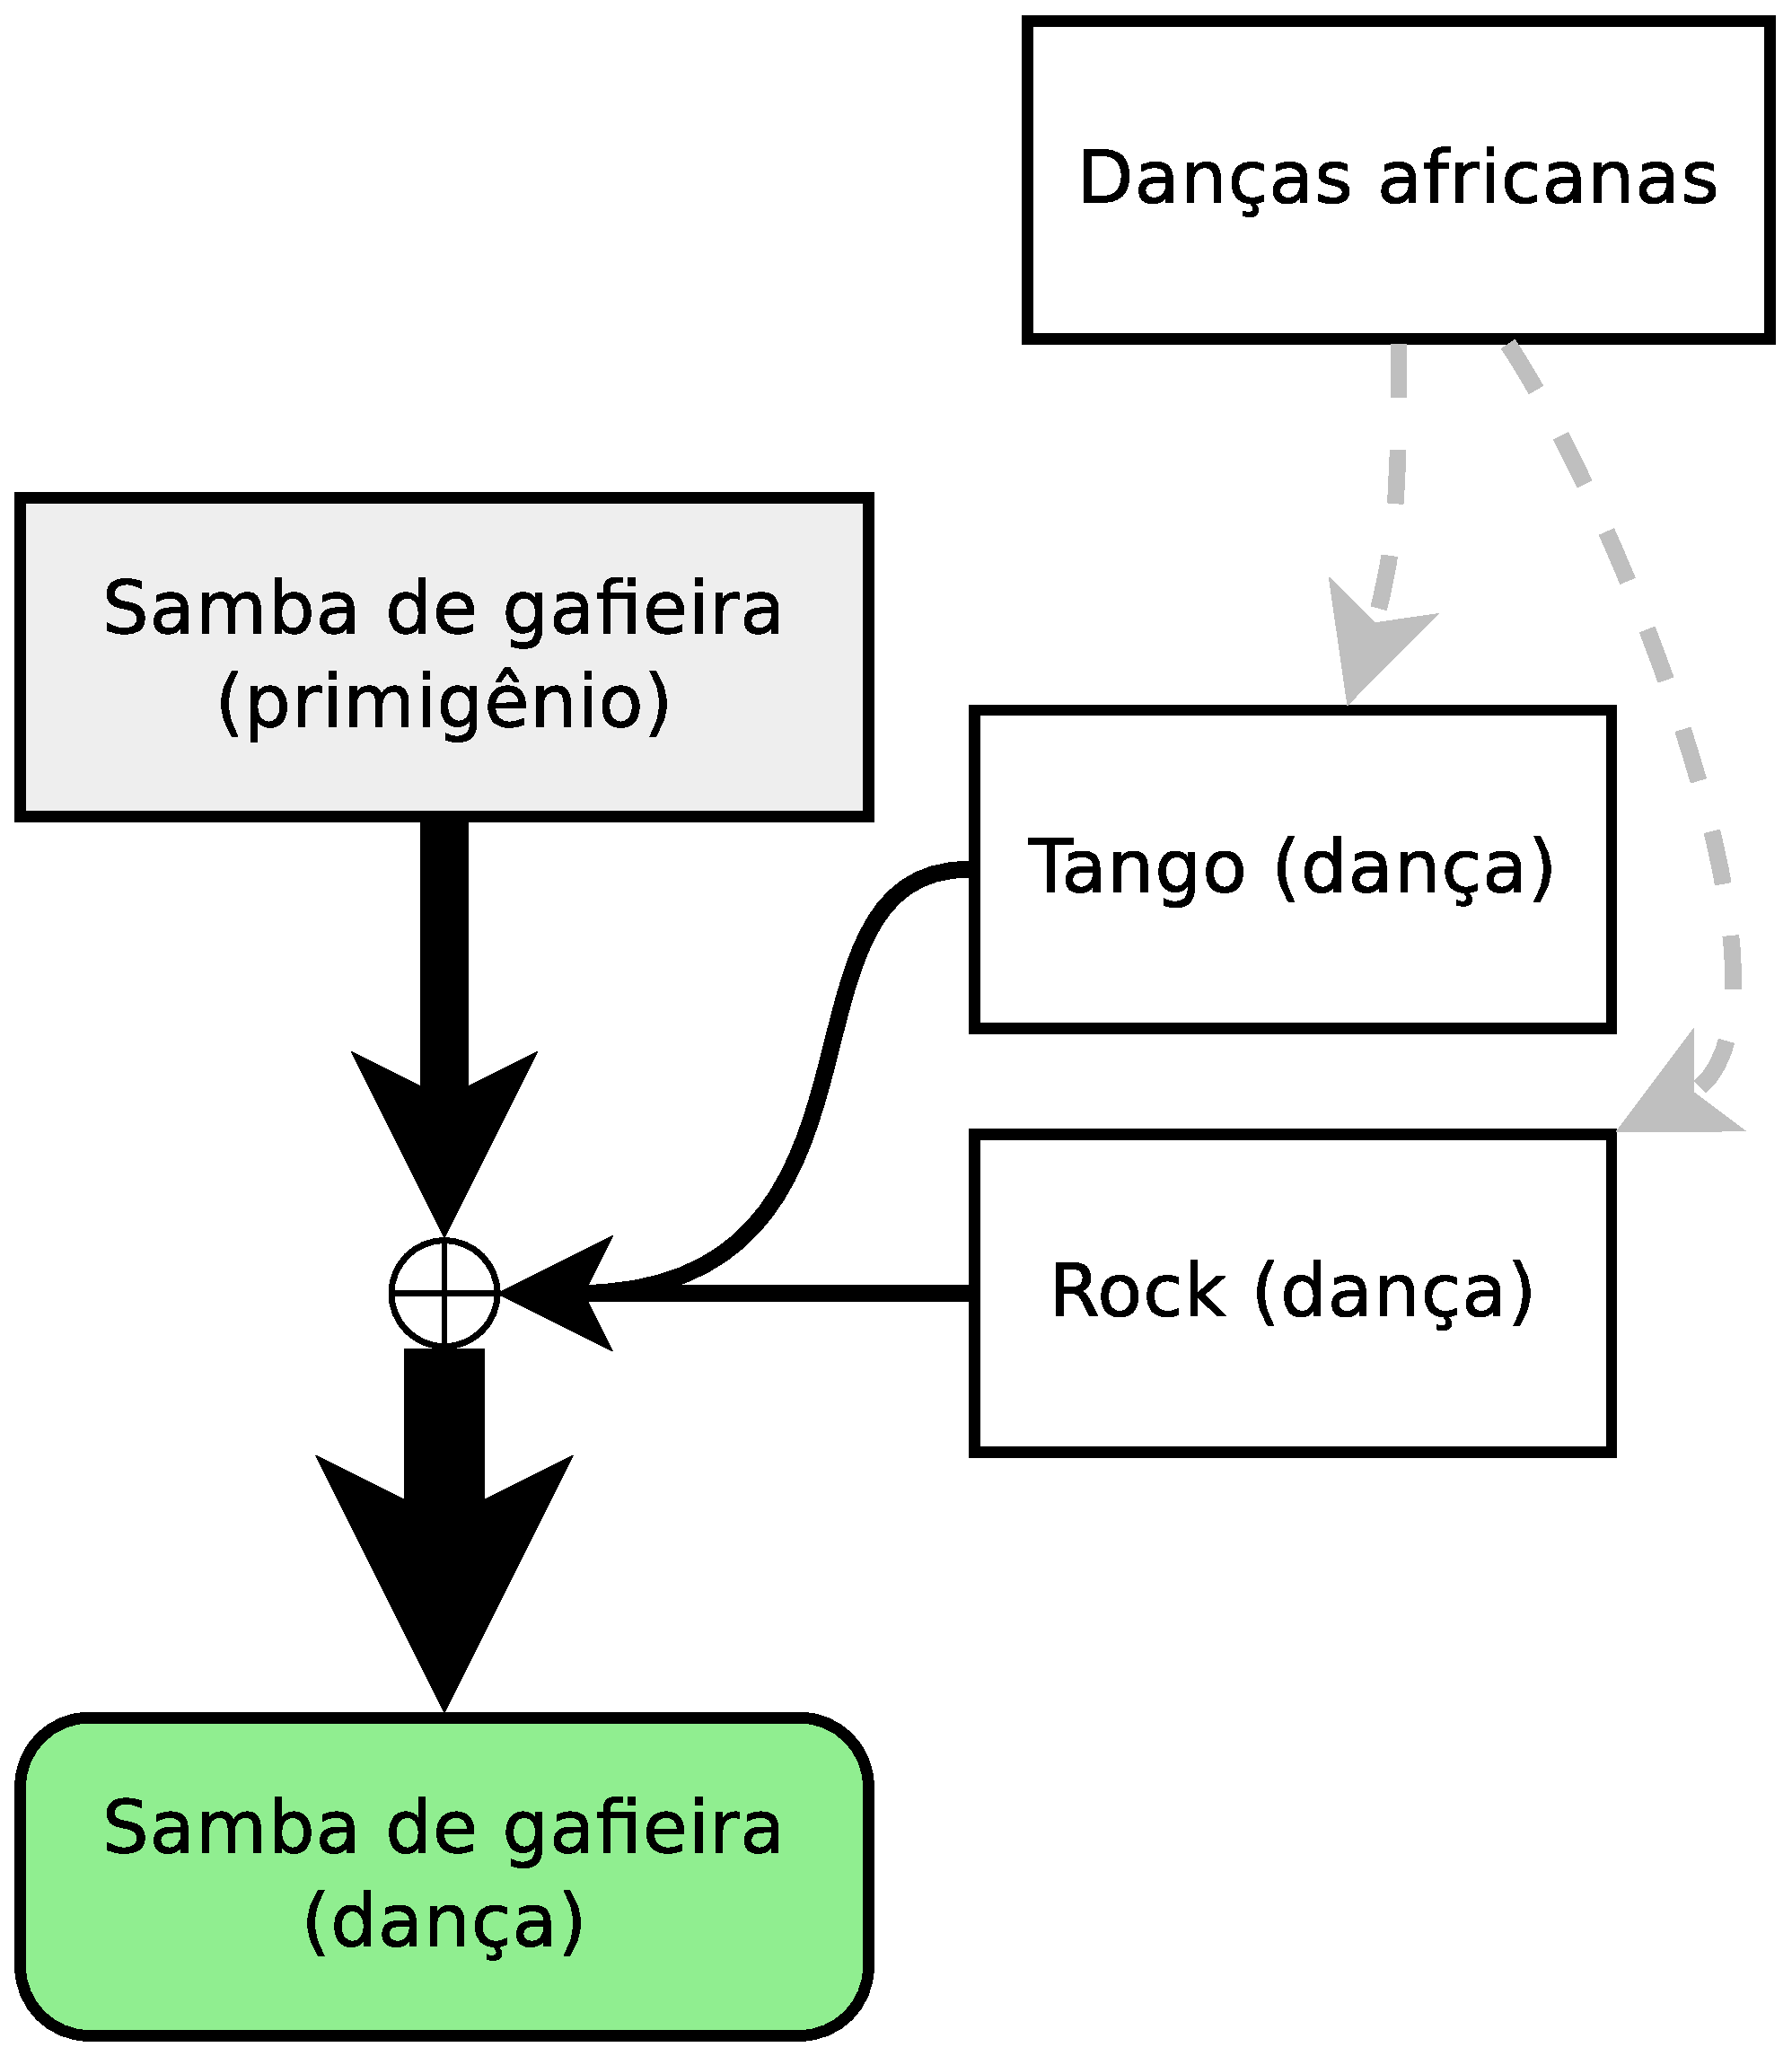
\includegraphics[width=\textwidth]{chapters/cap-historia-sambagafieira/sambagafieiraformula2.eps}
    \caption{Formação do samba de gafieira (atual).}
    \label{fig:formuladosambagafieira2}
  \end{subfigure}
\caption{Formula da criação do samba de gafieira.}
\label{fig:formuladosambagafieiraall}
\end{figure}


O aparecimento do samba nos salões de dança, 
foi um grande impacto para as pessoas que frequentavam estes lugares;
sendo considerado um ritmo novo e ligeiro,
que desagradou aos bailarinos de maior idade e menos ágeis \cite[pp. 6 - cad. B]{entrevistajuliojournalbrasil1}.
O senhor, Júlio Simões, socio da ``Kananga do Japão'' e
do ``Elite Club'', chegou a temer pelo futuro do seus empreendimentos; porem, para sorte dele, 
o samba fez muito sucesso no Elite,
e passou a ser considerado vestibular indispensável para qualquer pessoa que pretendesse ser bailarino, 
compositor ou instrumentista \cite[pp. 6 - cad. B]{entrevistajuliojournalbrasil1}.

\PRLsep{Samba nos salões em 1940}

Pode-se estabelecer o ingresso do samba, aos salões de dança, entre os anos de 1930 e 1940 \cite[pp. 140]{perna2002samba}.
Em palavras do Prof. de dança Gino Fornaciari, 
o samba dessa época tinha um aprecido com o Foxtrot e a Rumba, se dançava num compasso binario,
sendo esta dança a preferida do mulato brasileiro
%sendo este estilo de dança de salão que nasceu na \hyperref[ref:batucadadanca]{\textbf{batucada}} 
%de pretos que descia à cidade na epoca das festas 
\cite[pp. 50]{fornaciari1947aprender}.
Para a decada de 1940 o samba carioca de salão \cite[pp. 50]{fornaciari1947aprender},  já tinha ganhado muita força nos salões,
e podia-se ver 3 modalidades de dançar o samba \cite[pp. 58]{freitas1959danca} \cite[pp. 142-143]{perna2002samba} 
\cite[pp. 51]{fornaciari1947aprender}:
\begin{itemize}
\item \textbf{Samba-canção (dança)},
\index{Dança!Samba-canção} 
Era uma dança com balanços aos lados que se executava de joelhos flexionados,
usando dois movimentos por cada compasso binario \cite[pp. 58]{freitas1959danca} 
\cite[pp. 51]{fornaciari1947aprender} \cite[pp. 143]{perna2002samba}; 
na atualidade é um modo de dança extinto \cite[pp. 143]{perna2002samba}.

Sobre os passos usados entre 1947-1959, 
na Figura \ref{fig:samba-cancao-basico-frente} se mostra o passo básico para a frente do samba-canção,
e na  Figura \ref{fig:samba-cancao-basico-frente} o mesmo movimento para trás;
em ambos casos se usa os 2 movimentos antes mencionados, e a cor cinza indica a posição inicial \cite[pp. 51]{fornaciari1947aprender} \cite[pp. 59-60]{freitas1959danca}. 
\begin{figure}[h]
    \centering
    \begin{subfigure}[b]{0.3\textwidth}
        \centering
        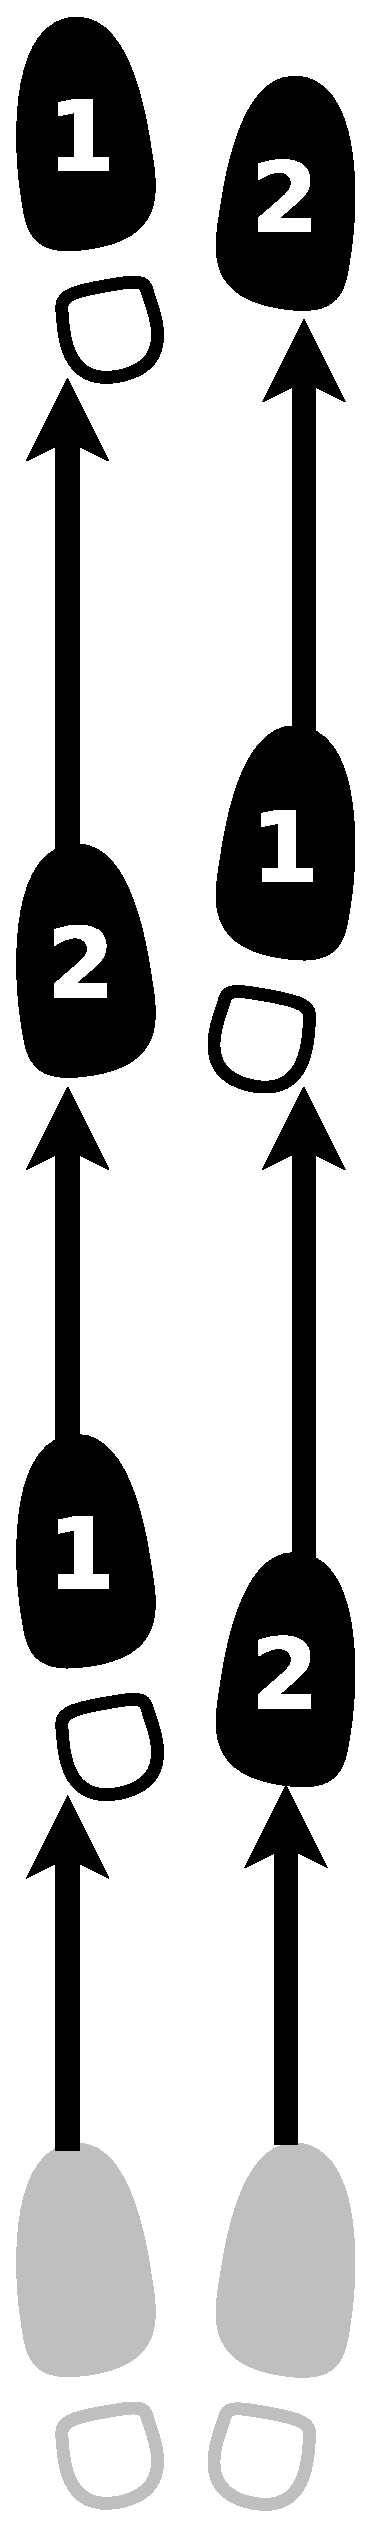
\includegraphics[width=0.2\textwidth]{chapters/cap-historia-sambagafieira/samba-cancao-basico-frente.eps}
        \caption{Passo básico para a frente.}
        \label{fig:samba-cancao-basico-frente}
    \end{subfigure}
    ~ %add desired spacing between images, e. g. ~, \quad, \qquad, \hfill etc. 
      %(or a blank line to force the subfigure onto a new line)
    \begin{subfigure}[b]{0.3\textwidth}
        \centering
	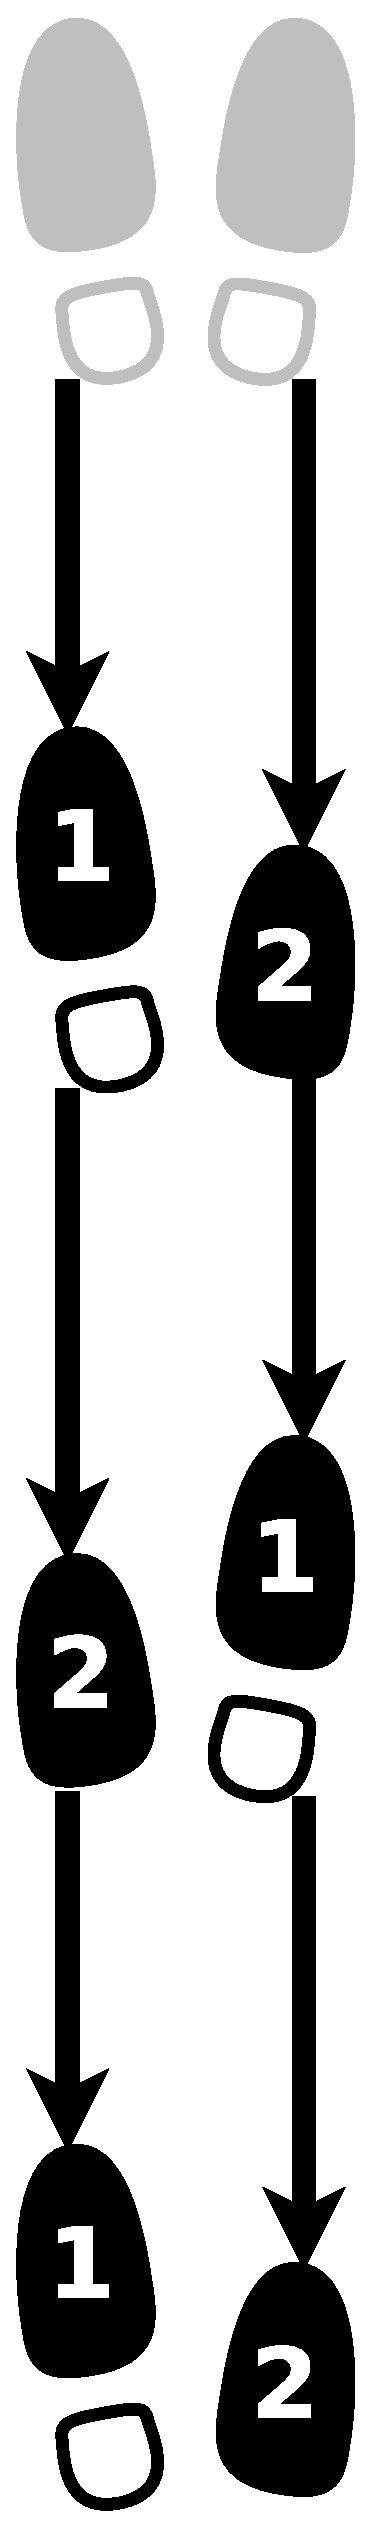
\includegraphics[width=0.2\textwidth]{chapters/cap-historia-sambagafieira/samba-cancao-basico-tras.eps}
        \caption{Passo básico para trás.}
        \label{fig:samba-cancao-basico-tras}
    \end{subfigure}
    \caption{Samba canção da década de 1959.}\label{fig:samba-cancao-basico}
\end{figure}


\item \textbf{Samba-batucada},
\index{Dança!Samba-batucada} 

O samba batucada é o samba de gafieira (primigênio) \cite[pp. 143]{perna2002samba}.

Existe uma menção sobre este estilo no ``Jornal do Brasil'', no dia 9 de janeiro de 1938,
onde se indica \cite[pp. 4]{musicasambavariasdef1}:
\begin{citando}%%
Tentativas isoladas de puro 
snobismo e ás vezes de compreensão 
inexata da origem da 
musica e dansa, chamam-no de samba jongo, \textbf{samba batucada} ou
pretendem mistura-lo com o fox, -- samba fox ou com a rumba samba-rumba.
\end{citando}



No livro ``Feitiço decente: Transformações do samba no Rio de Janeiro (1917-1933)'' (2001),
se comenta, sobre uma roda do samba, que para o dançarino solista  escolher a seu sucessor podiam
existir duas modalidades, em ``samba liso'' (com umbigada) ou em ``samba duro'' 
(ou batucada) no qual a umbigada é substituída por uma pernada \cite[pp. 109]{sandroni2001feitico}.
Deste comentário pode ser deduzido de onde vem a denominação \textbf{samba-batucada}, 
que surgiu nos salões de dança apos 1930; pois já existia uma tradição na nomenclatura,
em separar duas formas de dançar uma mais leve (a liso) e uma mais brusca (batucada);
assim, a variante de samba no salão que tendia a explorar movimentos muito  gingados, bruscos ou rápidos,
foi nomeado de samba-batucada, em contraposição ao samba liso onde né se flexionavam os joelhos pra dançar.  



O samba-batucada era, entre 1947 e 1959, uma dança com balanços que se dançava de joelhos flexionados  
e usava 3 movimentos por compasso, que exigia uma maior rapidez, 
especialmente no terceiro movimento que é mais rápido e curto \cite[pp. 61]{fornaciari1947aprender} \cite[pp. 58,66]{freitas1959danca};
seguindo essa descrição, 
o mais provável é que se dançara seguindo uma distribuição de tempos,
parecida ao ritmo do baião de 1949 \cite{CORTES2014}, como pode-se ver na Figura \ref{time:sambabatucada}.
\begin{figure}[H]
\centering
\begin{abc}[name=abc-sambabatucada]
X: 1 % start of header
K: C stafflines=1 % scale: C major
M: 2/4 %meter - compasso
%Q:1/4=100
V:1 clef=perc stem=up %name="TC"   sname="TC"
[V:1] |:  B3/2 B/2 B1 z1 | B3/2 B/2 B1 z1 | B3/2 B/2 B1 z1 | B3/2 B/2 B1 z1 :|
w:        P1   P2  P3      P1   P2  P3      P1   P2  P3      P1   P2  P3
\end{abc}
\caption{Frase de 8 tempos onde P1, P2 e P3 indicam o pé 1, 2 e 3 respetivamente.}
\label{time:sambabatucada}
\end{figure}

Sobre os passos usados na época, 
na Figura \ref{fig:samba-batucada-basico-frente} se mostra o passo básico para a frente do samba-batucada,
e na  Figura \ref{fig:samba-batucada-basico-tras} o mesmo movimento para trás;
em ambos casos se usa os 3 movimentos antes mencionados, e a cor cinza indica a posição inicial \cite[pp. 61-62]{fornaciari1947aprender} \cite[pp. 63]{freitas1959danca}. 
\begin{figure}[h]
    \centering
    \begin{subfigure}[b]{0.3\textwidth}
        \centering
        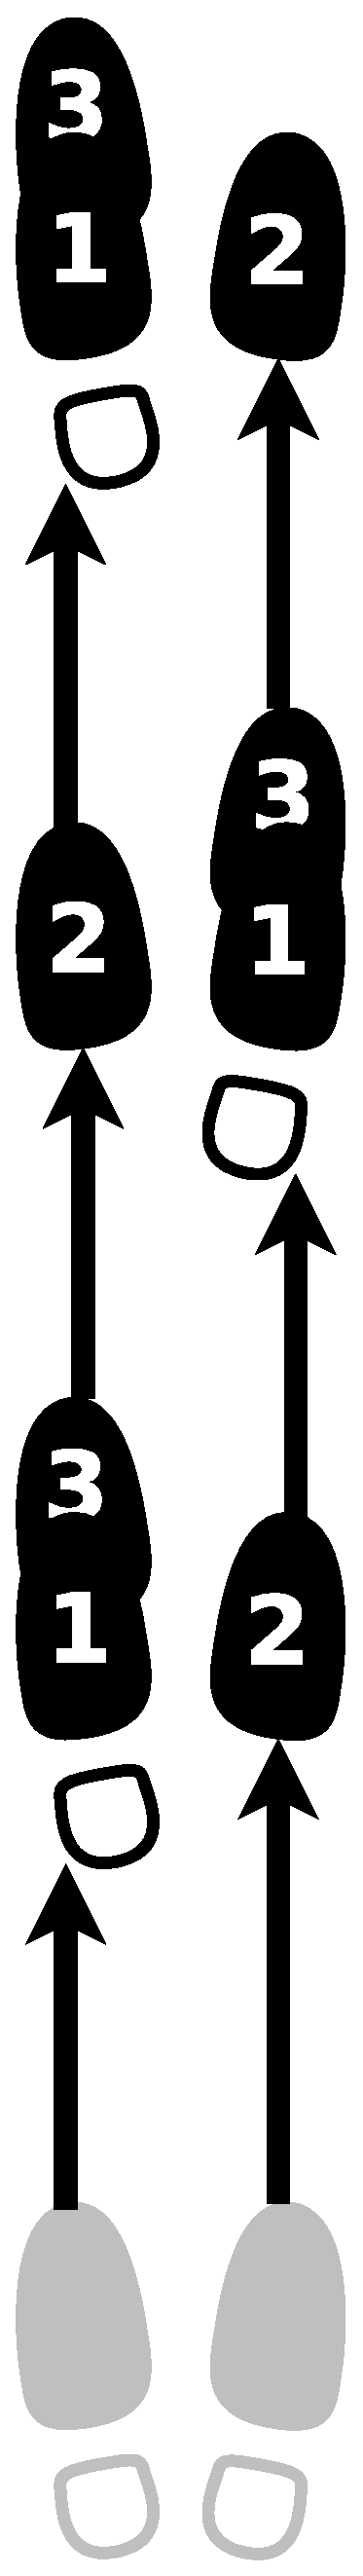
\includegraphics[width=0.2\textwidth]{chapters/cap-historia-sambagafieira/samba-batucada-basico-frente.eps}
        \caption{Passo básico para a frente.}
        \label{fig:samba-batucada-basico-frente}
    \end{subfigure}
    ~ %add desired spacing between images, e. g. ~, \quad, \qquad, \hfill etc. 
      %(or a blank line to force the subfigure onto a new line)
    \begin{subfigure}[b]{0.3\textwidth}
        \centering
	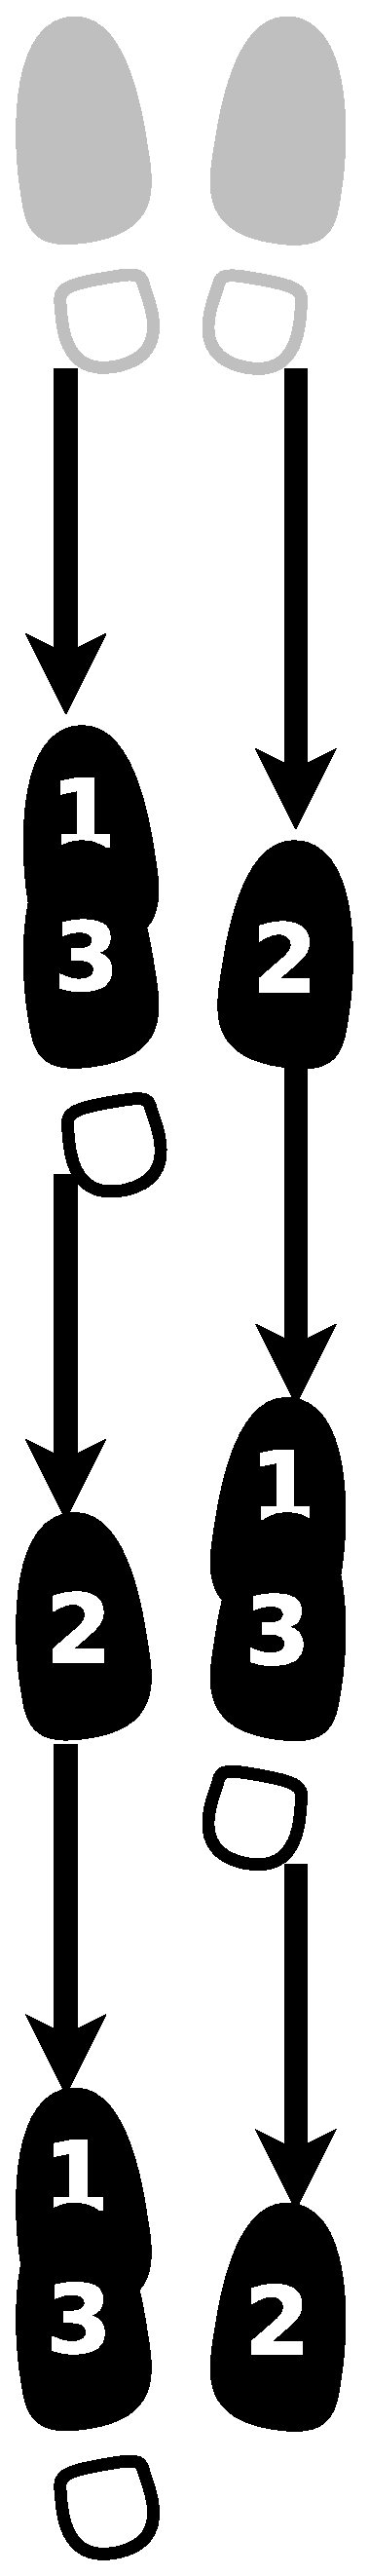
\includegraphics[width=0.2\textwidth]{chapters/cap-historia-sambagafieira/samba-batucada-basico-tras.eps}
        \caption{Passo básico para trás.}
        \label{fig:samba-batucada-basico-tras}
    \end{subfigure}
    \caption{Samba batucada da década de 1959.}\label{fig:samba-batucada-basico}
\end{figure}

Outros passos conhecidos no ano de 1947, para este estilo de samba, tem nomes como: 
o pião, o balão, a cortada, a meia cortada, a joelhada, a patineta, e outros \cite[pp. 66]{fornaciari1947aprender};
porem, seguindo o Prof. Fornaciari, o pião e o balão são o mesmo movimento, 
sendo este o movimento mais importante do samba batucada;
e a diferença do pião atual que se executa tradicionalmente em sentido horário,
o pião de 1947 se executava em sentido anti-horário \cite[pp. 68,72]{fornaciari1947aprender}.




\item \textbf{Samba liso}, 
\index{Dança!Samba liso}
Era uma dança com balanços que se dançava sem flexionar os joelhos;
este é um estilo de dança que perdura ainda ate nossos 
dias \cite[pp. 58,62]{freitas1959danca} \cite[pp. 143]{perna2002samba}, 
para mais detalhes ver a Seção \ref{subsec:estilosdedancapares}.
\end{itemize}

\subsection{Evolução do samba nos salões}

Com o passar dos anos foram agregados elementos de outras danças a esse primitivo, samba de gafieira;
por exemplo, movimentos do tango e do rock \cite[pp. 142]{perna2002samba}, 
obtendo assim a forma de dança que vemos hoje em dia, ver Figura \ref{fig:formuladosambagafieira2}.

Asim, podemos falar do samba de gafieira como dança, só apos da aparição do samba nos
salões de dança abertos ao público, e a partir da criação do termo gafieira pra definir a estes lugares.
Com a mistura destes dois acontecimentos obtemos o termo, samba de gafieira,
que iniciou seu caminho na dança, mas como uma descrição do âmbito da dança (e da música), que como nome próprio.
Porem, a formação dos movimentos e corporalidade desta dança tem um caminho que data desde muito tempo atrás,
desde os batuques, dos morros e das rodas.


A primeira referencia achada\footnote{Que não quer dizer a primeira existente.} 
na ``Hemeroteca Digital Brasileira'' da Fundação Biblioteca Nacional,
foi na ``Revista da Semana''(RJ), no dia 25 de dezembro de 1948,
onde na seção ``Eros Volusia'', subseção ``O pitoresco da excursão'', se indica \cite[pp. 48]{sambagafieirarefbn}
\begin{citando}
Ensinando o samba aos ministros da República, 
fazendo o povo vibrar com o \textbf{samba de gafieira}, entusiasmando
o meio intelectual com seu francês muito doce,
contando coisas desconhecidas aos dançarinos francêses,
fazendo a dança brasileira figurar nos Archives Internationales de la Danse.
Eros Volusia satisfez o grande ideal de sua vida artística, sentindo-se contente
com o que realizou na França, embora a Europa não dê dinheiro a ninguém.
O lucro artístico é que compensa.
\end{citando}


A Figura \ref{fig:sambagafieiracrono} mostra a cronologia do uso do termo samba de gafieira. 

\begin{figure}[h]
  \centering
    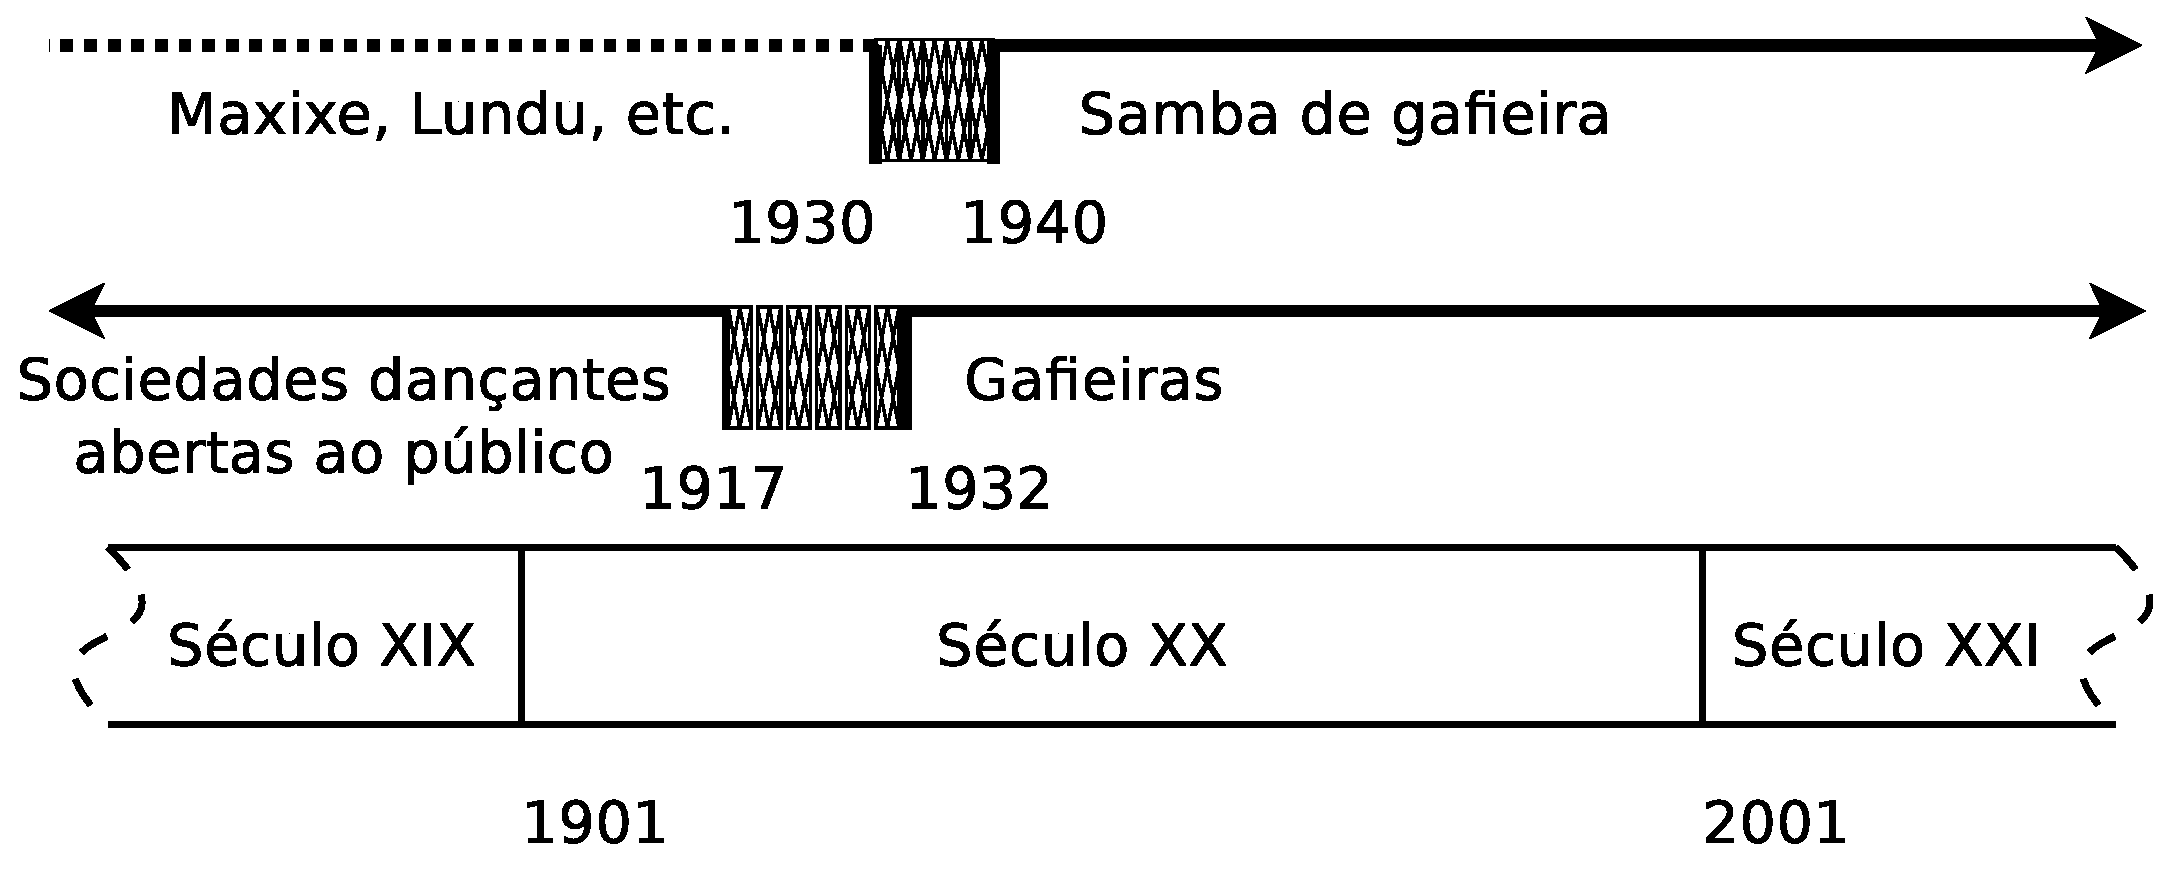
\includegraphics[width=0.7\textwidth]{chapters/cap-historia-sambagafieira/gafieira-crono.eps}
  \caption{ Cronologia da formação do samba de gafieira.}
\label{fig:sambagafieiracrono}
\end{figure}

%%%%%%%%%%%%%%%%%%%%%%%%%%%%%%%%%%%%%%%%%%%%%%%%%%%%%%%%%%%%%%%%%%%%%%%%%%%%%%%
\section{\textcolor{blue}{Em que estilos musicais posso dançar samba de gafieira?}}
\label{subsec:gafieiradancaestilos}

Entre os estilos musicais em que o samba de gafieira se adapta bem, temos:
\begin{itemize}
\item \textbf{Samba de gafieira (música)}

\item \textbf{Samba de breque}
\begin{example} ~
\begin{itemize}
\item ``Baile no elite'' interpretado por Casuarina.
\item ``Eu sou a marrom'' interpretado por Alicione.
\item ``Hoje sou diferente'' interpretado por Lenita Rodrigues.
\item ``Pra levantar poeira'' interpretado por Bodhar.
\end{itemize}
\end{example} 

\item \textbf{Pagode paulista}

\item \textbf{Partido alto}
\begin{example} ~
\begin{itemize}
\item ``A língua'' interpretado por Beto lima.
\item ``Partido Alto'' interpretado por Aleh.
\end{itemize}
\end{example} 

\item \textbf{Pagode (carioca)}
\begin{example} ~
\begin{itemize}
\item ``Trilha Do Amor''  interpretado pelo Grupo Revelação. 
\item ``A Batucada Te Pegou'' interpretado pelo Grupo Sou Muleke.
\item ``Dança da Solidão'' interpretado por Pagode de Mesa do álbum Terra Brasil. 
\item ``Eu e você sempre'' interpretado por Jorge Aragão
\end{itemize}
\end{example} 

\item \textbf{Samba canção}
\begin{example} ~
\begin{itemize}
\item ``Eu Quero E Sossego'' interpretado por Paulo Moura.
\item ``So Louco'' interpretado por Luiz Melodia.
\item ``Você É a Fonte'' interpretado por  Quinteto em Branco e Preto.
\item ``Eu Quero é Sossego'' interpretado por Paulo Moura.
\end{itemize}
\end{example} 

\item \textbf{Bossa nova}
\begin{example} ~
\begin{itemize}
\item ``I Don't Know (Bossa Mix)'' interpretado por Erika do álbum ``I Don't Know''
\item ``Human Nature'' interpretado por Marcela Mangabeira.
\end{itemize}
\end{example} 


\item \textbf{Choro}
\begin{example} ~
\begin{itemize}
\item ``Choro de gafieira'' de Pixinguinha.
\item ``Chorinho de gafieira'' de Astor Silva.
\item ``Noites Cariocas'' de Jacob do Bandolim.
\end{itemize}
\end{example} 


\item \textbf{Samba-choro}
\begin{example} ~
\begin{itemize}
\item ``Escurinho'' interpretado por Corina Magalhães.
\end{itemize}
\end{example}

\end{itemize}

A Figura \ref{fig:gafieiradancaestilos} mostra um resumo dos 
tipos de estilos musicais onde pode ser dançado samba de gafieira.
\begin{figure}[h]
  \centering
    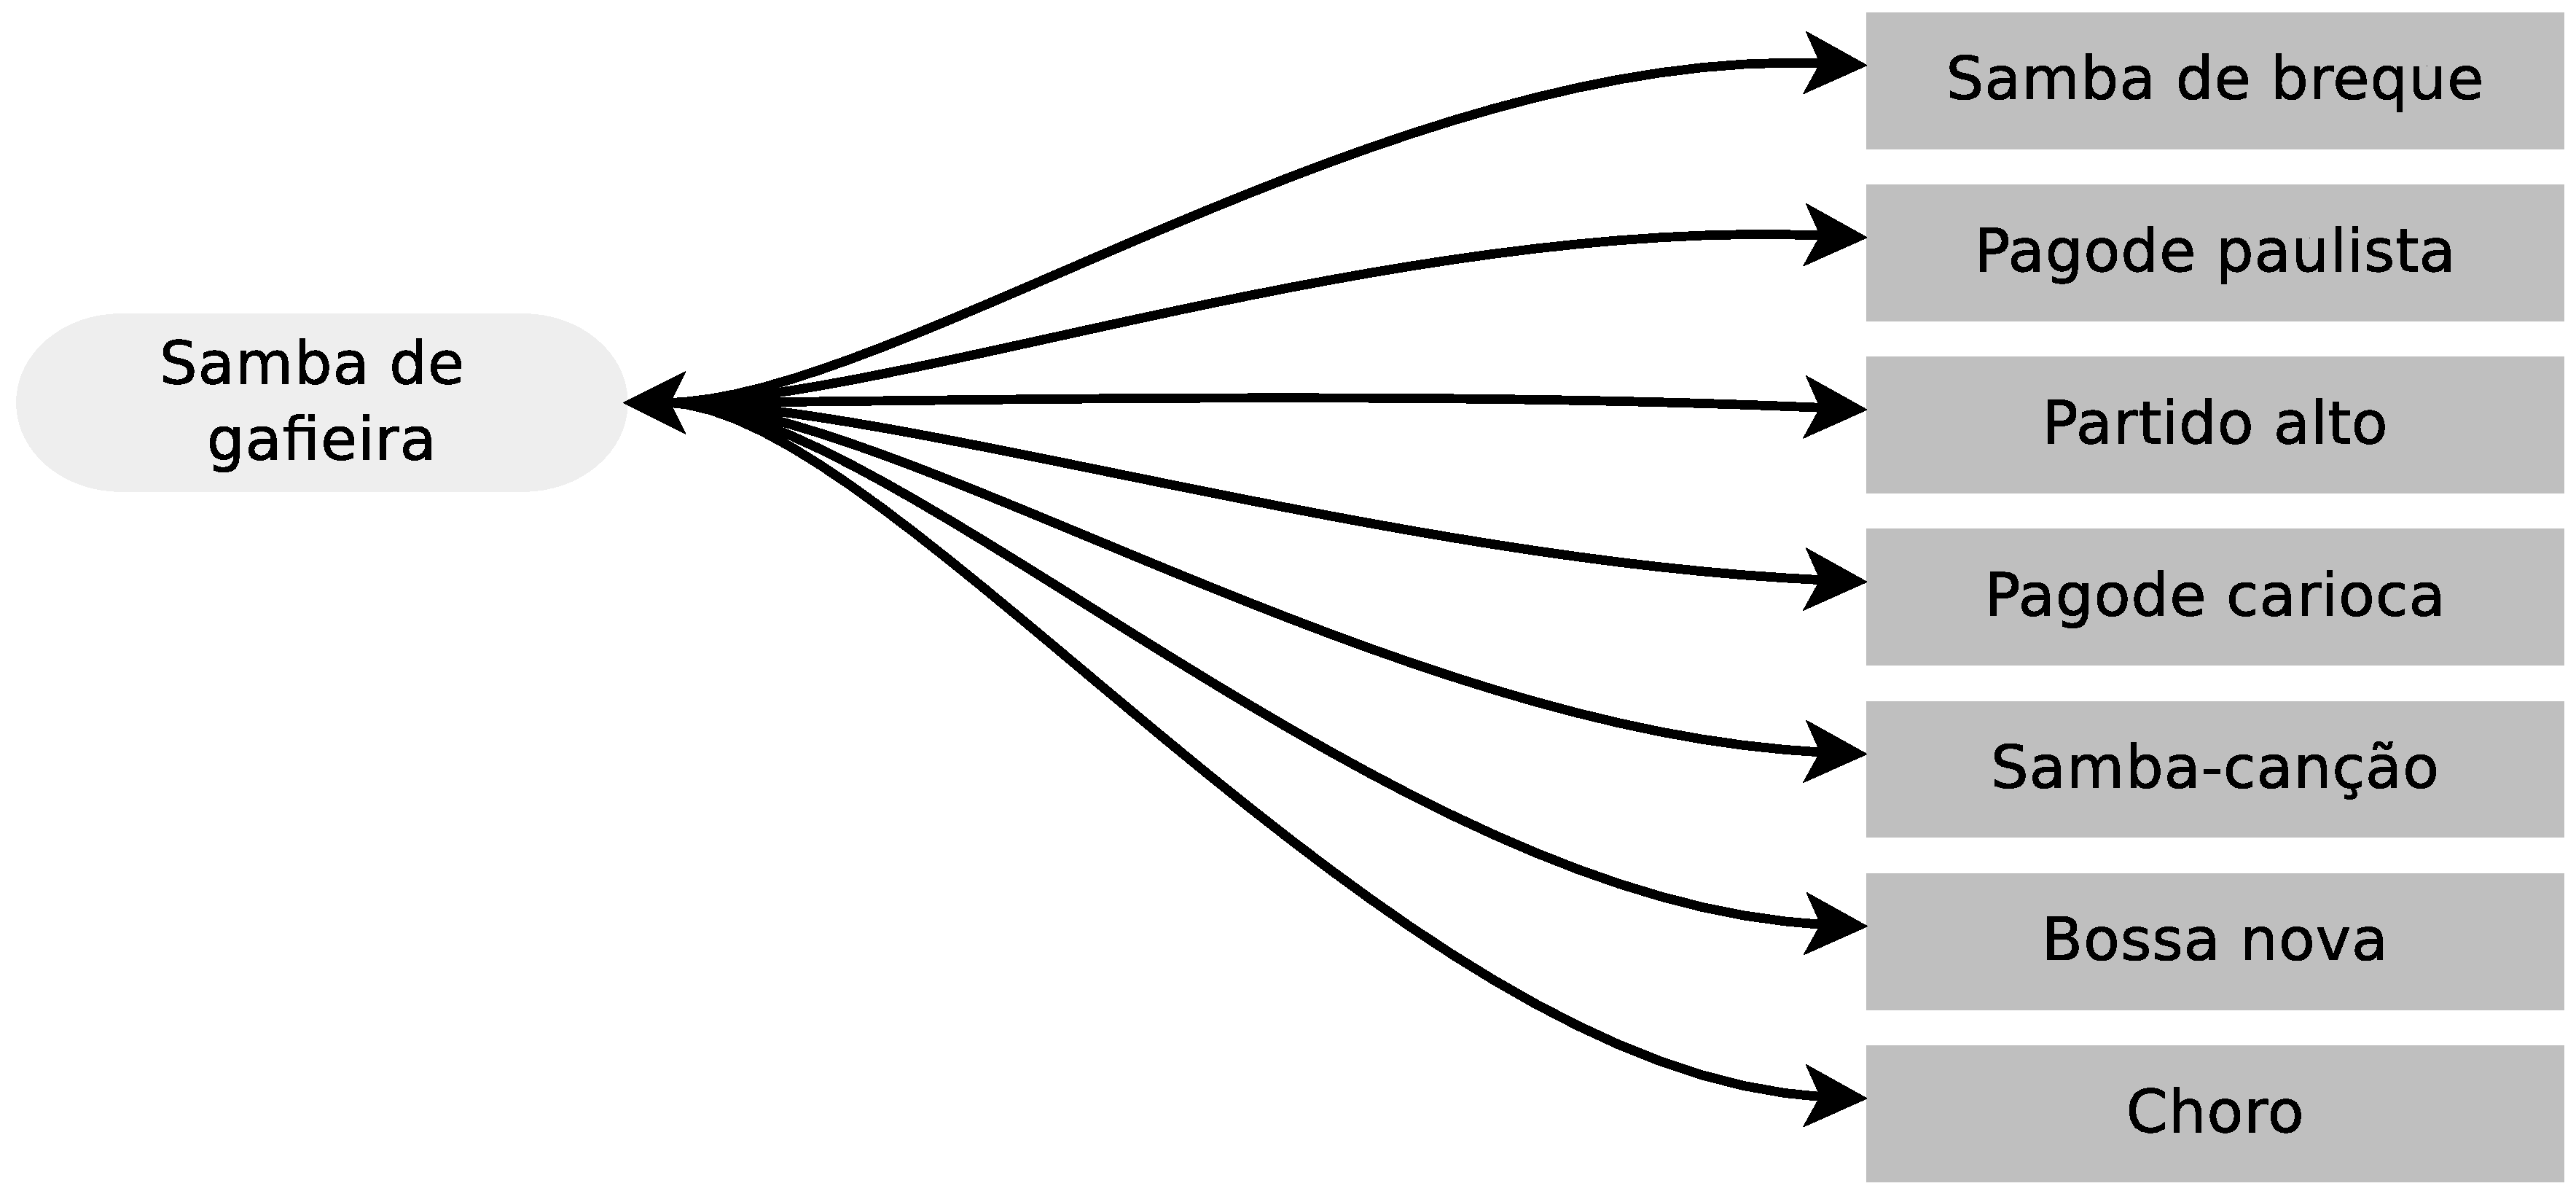
\includegraphics[width=0.6\textwidth]{chapters/cap-historia-sambagafieira/gafieiravcmusica.eps}
  \caption{ Estilos de músicas no samba onde pode-se dançar samba de gafieira.}
\label{fig:gafieiradancaestilos}
\end{figure}

